\documentclass[a4paper]{article}
\setlength{\headheight}{1.1\baselineskip}
\usepackage[english]{babel}
\usepackage[utf8x]{inputenc}
% package for including graphics with figure-environment
\usepackage{graphicx}
\usepackage{hyperref}
% colors for hyperlinks
% colored borders (false) colored text (true)
\hypersetup{colorlinks=true,citecolor=black,filecolor=black,linkcolor=black,urlcolor=black}

% package for bibliography
\usepackage[authoryear,round]{natbib}
% package for expectation signs
\usepackage{amsmath,amssymb,mathtools,bm,etoolbox}
%\documentclass[a4paper,11pt]{report} 
\usepackage{breqn}
\usepackage{amsmath}
\usepackage{enumitem} 
\usepackage{amsmath, amsthm, amssymb}
\usepackage{amsmath}
\newcommand{\abs}[1]{ \left\lvert#1\right\rvert} 
\newcommand{\norm}[1]{\left\lVert#1\right\rVert}

% some more packages enabling table and figure production
\usepackage{float, afterpage, rotating, graphicx}
\usepackage{epstopdf}
\usepackage{longtable, booktabs, tabularx}
\usepackage{fancyvrb, moreverb, relsize}
\usepackage{eurosym, calc, chngcntr}
\usepackage{amsmath, amssymb, amsfonts, amsthm, bm}
\usepackage{caption}
\usepackage{mdwlist}
\usepackage{xfrac}
\usepackage{setspace}
\usepackage{xcolor}
\usepackage{multirow}

\begin{document}
\begin{table}[H]
\caption {Mean Squared Error Comparison} \label{tab:mean squared error}

(standard normal distribution for $x_1$, $x_2$)

\begin{tabular}{l r r}

\toprule
 & \textbf{Standard Normality} & \textbf{Joint Normality} \tabularnewline\midrule
Ichimura's Model & 0.0020 & 0.0032
\tabularnewline
Klein and Spady's Model & 0.000089 & 0.00023
\tabularnewline 
Logit Model & 0.00092  & 0.0012
\tabularnewline
\bottomrule
\end{tabular}
\end{table}

\begin{figure}[h!]
  \caption{Plot of Estimates}
  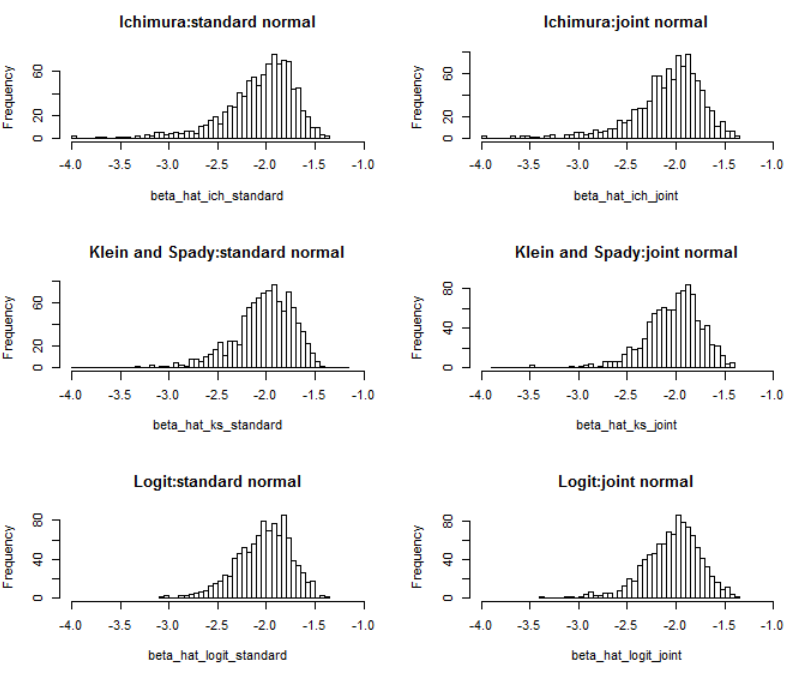
\includegraphics[width=\linewidth]{plot_comparison.png}
 
  \label{fig:plot of estimates}
\end{figure}

\end{document}